\documentclass[12pt]{report}
\usepackage{polski}
\usepackage[utf8]{inputenc}
\usepackage[a4paper]{geometry}
\usepackage[myheadings]{fullpage}
\usepackage{fancyhdr}
\usepackage{lastpage}
\usepackage{graphicx, wrapfig, subcaption, setspace, booktabs}
\usepackage[T1]{fontenc}
\usepackage[font=small, labelfont=bf]{caption}
\usepackage{fourier}
\usepackage[protrusion=true, expansion=true]{microtype}
\usepackage{sectsty}
\usepackage{url, lipsum}
\usepackage{tgbonum}
\usepackage{hyperref}
\usepackage{xcolor}
\usepackage{listings}
\usepackage{color}
\usepackage{float}


\definecolor{codegreen}{rgb}{0,0.6,0}
\definecolor{codegray}{rgb}{0.5,0.5,0.5}
\definecolor{codepurple}{rgb}{0.58,0,0.82}
\definecolor{backcolour}{rgb}{0.95,0.95,0.92}
 
\lstdefinestyle{mystyle}{
    backgroundcolor=\color{backcolour},   
    commentstyle=\color{codegreen},
    keywordstyle=\color{magenta},
    numberstyle=\tiny\color{codegray},
    stringstyle=\color{codepurple},
    basicstyle=\footnotesize,
    breakatwhitespace=false,         
    breaklines=true,                 
    captionpos=b,                    
    keepspaces=true,                 
    numbers=left,                    
    numbersep=5pt,                  
    showspaces=false,                
    showstringspaces=false,
    showtabs=false,                  
    tabsize=2
}

\lstset{style=mystyle}
\makeatletter

\renewcommand{\thesection}{%
  \ifnum\c@chapter<1 \@arabic\c@section
  \else \thechapter.\@arabic\c@section
  \fi
}
\makeatother
\newcommand{\code}[1]{\texttt{#1}}
\newcommand{\HRule}[1]{\rule{\linewidth}{#1}}
\onehalfspacing
\setcounter{tocdepth}{5}
\setcounter{secnumdepth}{5}
\pagestyle{fancy}  
\fancyhf{}
\chead{Sprawozdanie końcowe, grupa 3}
\cfoot{Strona \thepage/\pageref{LastPage}}
\graphicspath{ {images/} }
\begin{document}
{\fontfamily{cmr}\selectfont
\title{ \normalsize \textsc{}
		\\ [2.0cm]
		\HRule{0.5pt} \\
		\LARGE \textbf{{Sprawozdanie końcowe grupa 3}
		\HRule{0.5pt} \\ [0.5cm]
		\normalsize \today \vspace*{5\baselineskip}}
		}
}

\date{}

\author{
		Krzysztof Anderson i Michał Malinowski \\ }

\maketitle\thispagestyle{fancy}
\tableofcontents\thispagestyle{fancy}
\newpage

\sectionfont{\scshape}
\section{Wstęp teoretyczny}
„Gra w życie” brytyjskiego matematyka Johna Conwaya jest jednym z pierwszych i najbardziej znanych przykładów automatu komórkowego. Została wymyślona w 1970 roku i wzbudziła duże zainteresowanie z powodu zaskakującego sposobu, w jaki struktury powtrafią ewoluować. Fizyków inspirowała do tworzenia symulacji, a matematykom dawała dużo możliwości (np. niektóre struktury mogą być wykorzystywane do generowania liczb pierwszych.).\par
Gra polega na ustalaniu stanów poszególnych komórek na planszy gry, w~zależności od stanu wszystkich komórek sąsiadujących. \par
Na potrzeby programu plansza składa się ze skończonej ilości pól, na której będą tworzone nowe generacje. Plansza składa się z 0 i 1. 0 reprezentują komórki martwe, a 1 żywe.\par
Komórka pozostaje żywa jeżeli posiada 2 lub 3 sąsiadów.\par
Komórka ożywa, jeżeli ma 3 żywych sąsiadów.\par
Stany wszystkich komórek zamieniają się dopiero po ustaleniu dla wszystkich komórek, jaki stan przyjmie w następnej generacji.
\section{Osiągnięte cele}
Program spełnia wszystkie wymagania, jakie zostały zawarte w specyfikacjach. Program potrafi
\begin{itemize}
    \item wczytywać z pliku tekstowego początkowe ustawienie żywych komórek na planszy i potrafi przeprowadzić na nich zadaną ilość generacji.
    \item wypisywać na ekran obecną generację, wedle założeń zawartych w specyfikacji funkcjonalnej.
    \item wygenerować plik PNG reprezentujący graficznie ustawienie żywych komórek na aktualnej planszy.
    \item wygenerować plik tekstowy reprezentujący aktualne ustawienie żywych komórek na planszy, z założeniem, aby tworzony plik mógł zostać później wczytany jako plik startowy w omawianym programie.
    \item obsłużyć flagę „Step-by-step”. Wtedy zatrzymuje swoje działanie po wygenerowaniu każdej generacji i pyta użytkownika, czy chce zobaczyć kolejną generację, czy obecną wyeksportować do pliku PNG lub tekstowego, czy może zakończyć działanie programu na tej generacji.
    \item stworzyć plik wynikowy o poprawnej nazwie podanej przez użytkownika.
    \item obsługiwać błędy związane z podaniem niepoprawnych danych wejściowych, błędnych argumentów wywołania oraz błędnych nazw poleceń i nazw generowanych plików.
\end{itemize}
\section{Co zostało zmienione względem specyfikacji}
\begin{itemize}
    \item Typ funkcji \code{read\_board} został zamieniony z \code{void} na \code{int}, aby dostawać informację zwrotną, czy udało się poprawnie przeczytać plik. Funkcja zwraca 0 jeżeli uda się przeczytać i liczbę różną od 0 jeżeli się nie powiedzie.
    \item Definicja struktury \code{playboard} została przeniesiona do pliku nagłówkowego \code{gra.h}, aby nie było potrzeby deklarowania jej dwa razy.
    \item W definicji \code{playboard} znajduje się zapis \code{*playboard} zamiast \code{playboard*}, ponieważ stary zapis jest niepoprawny.
    \item Za flagę „Step-by-step” odpowiada funkcja \code{play}, zamiast \code{make\_generation}, gdyż jest to bardziej czytelne.
    \item Została dodana funkcja \code{void swapPtr} w \code{gra.c}, która odpowiada za zamianę wskaźników z głównej na pomocniczą i z pomocniczej na główną. Zmiana została dodana dla lepszej czytelności kodu.
    \item Typ funkcji \code{check\_filename} został zmieniony z \code{int} na \code{bool}, ponieważ funkcja i tak zwracała 0 lub 1.
    \item Została dodana funkcja \code{bool is\_number} do pliku \code{sterowanie.c}, aby sprawdzać czy argument podany jako ilość generacji jest liczbą. Zwraca \code{true} jeżeli jest i \code{false} jeżeli nie jest.
    \item Sposób wydawania komend podczas generowania "Step-by-step" uległ zmianie. Aktualnie nie ma potrzeby naciskania ENTER po wpisaniu każdego polecenia. Znacząco to ułatwia operowanie programem.
    \item W związku z powyższą zmianą uległy także zmianom komendy użytkownika.
    \begin{itemize}
        \item Należy wcisnąć \textbf{n}, aby przejść do następnej generacji.
        \item Należy wcisnąć \textbf{p}, aby zapisać aktualną generację do pliku PNG.
        \item Należy wcisnąć \textbf{t}, aby zapisać aktualną generację do pliku tekstowego. 
    \end{itemize}
    \item Została dodana opcja wyjścia z programu w trakcie generowania kolejnych generacji przy zapalonej fladze "Step-by-step". Aby ją wybrać należy wcisnąć \textbf{q}. Jest to bardzo przydatne podczas generowania dużej ilości generacji, gdy nagle chcemy zamknąć program.
    \item Sposób wyświetlania obecnej generacji na ekranie uległ zmianie. Aktualnie jedną komórkę na planszy reprezentują 2 znaki na ekranie. Zmiana została wprowadzona, ze względów estetycznych.
    \item Program wykonywalny został przeniesieniony do folderu bin, dla czytelności struktury programu.

\end{itemize}
\newpage
\section{Przykłady uruchomienia}
W tym rodziale zaprezentowane zostaną przykładowe wywołania programu z~różnymi parametrami. Pokazane zostaną wyniki użycia poszczególnych komend.
\begin{enumerate}
    \item Wywołanie programu komendą \code{bin/gra\_w\_zycie dane/pulsar.txt 4}\par
    \begin{figure}[H]
    \centering
    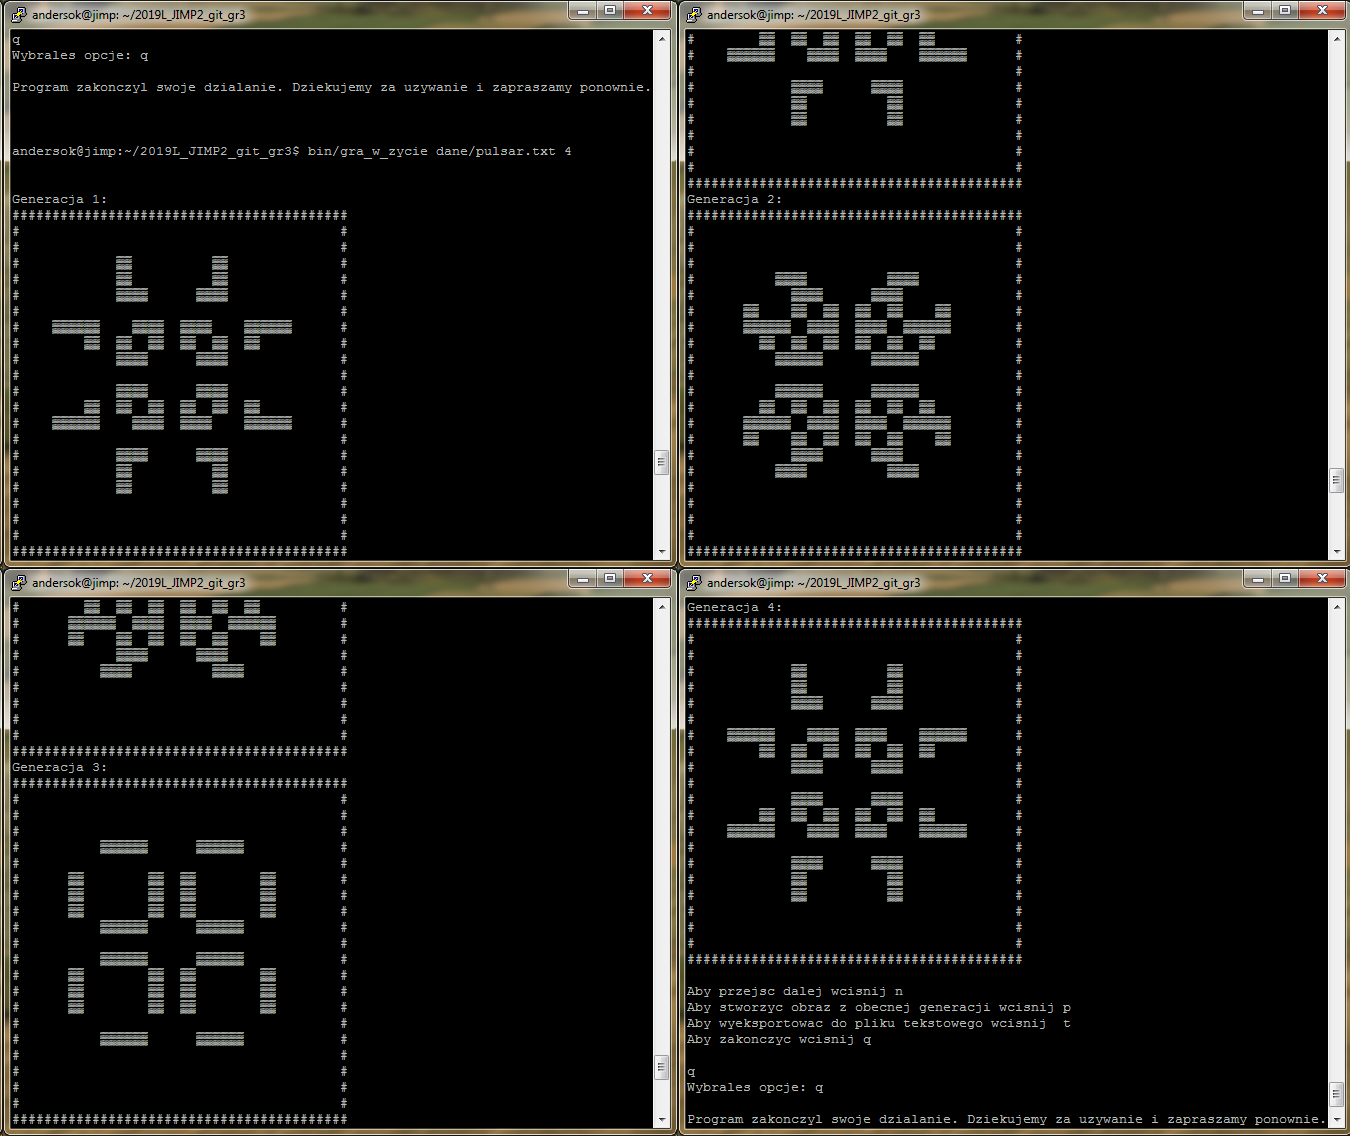
\includegraphics[width=14cm]{obrazy/przykladuzycia_1.png}
    \caption{Przykład użycia 1}
    \label{przyklad uzycia 1}
    \end{figure}\par
    Program zostaje uruchomiony na pliku pulsar.txt znajdującym się w pliku dane, który zawiera stan początkowy struktury oscylatorowej o nazwie "Pulsar". Struktura ta przekształca się, a po 4 generacjach wraca do swojego stanu początkowego. Zostają utworzone 4 generacje wczytanej planszy i kolejno wypisane na ekran. Po wypisaniu ostatniej generacji zostaje wyświetlone pytanie, czy pokazać następną generację (w tym przypadku nie ma już następnej, dlatego program zakończy swoje działanie), czy zapisać obecną generację do pliku tekstowego lub pliku PNG, czy zakończyć program. Zostaje wybrana opcja \textbf{q}, czyli zakończenie pracy programu. Na koniec można zaobserwować pożegnalny komunikat.
    \item Wywołanie programu komendą \code{bin/gra\_w\_zycie dane/pulsar.txt 8}\par
    \begin{figure}[H]
    \centering
    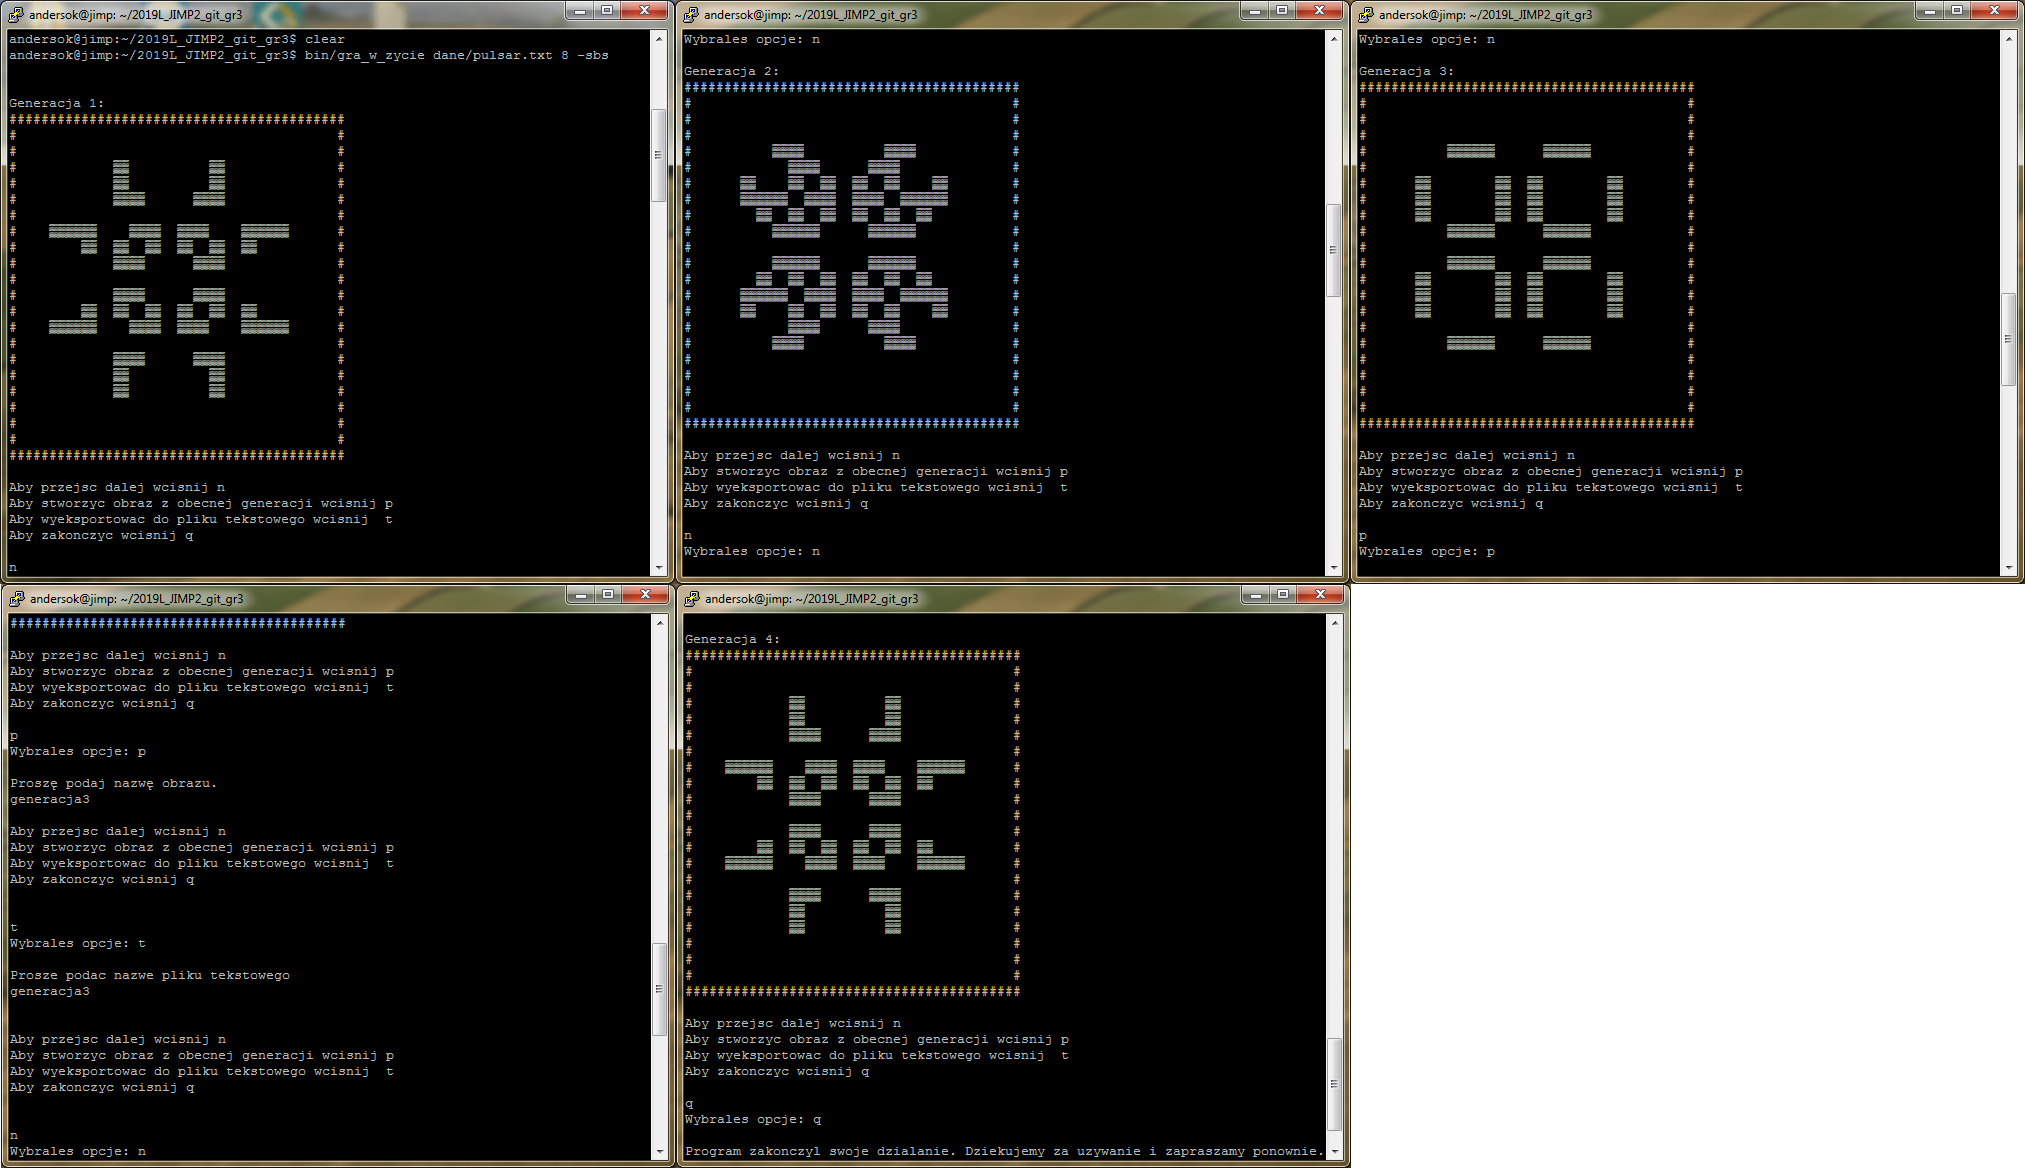
\includegraphics[width=14cm]{obrazy/przykladuzycia_2.png}
    \caption{Przykład użycia 2}
    \label{przyklad uzycia 2}
    \end{figure}\par
    Program zostaje uruchomiony na pliku pulsar.txt znajdującym się w pliku dane. Tym razem, podczas wywołania zostaje zapalona flaga "Step-by-step". Program po wygenerowaniu każdej generacji wyświetla pytanie, czy wygenerować następną generację, czy zapisać aktualny stan do pliku tekstowego lub PNG, czy może zakończyć działanie programu na obecnej generacji. Wykorzystując opcje przechodzenia dalej powstają 3 kolejne generacje. Wykorzystując dostępne funkcje, zostaje utworzony obraz PNG z zapisem trzeciej generacji o nazwie "generacja3.png". Następnie zostaje utworzony plik tekstowy o nazwie "generacja3.txt" również z zapisem tej samej generacji. Po przejściu do 4 generacji można zauważyć, że struktura wróciła do stanu początkowego i nie ma potrzeby przechodzenia do kolejnych generacji (będą one wyglądały tak samo jak te dotychczas wygenerowane). Dzięki wykorzystaniu odpowiedniej komendy, program kończy swoje działanie zanim zostanie wygenerowana zadana przez użytkownika liczba generacji.
\end{enumerate}
\section{Testowanie}
\par Na potrzebę przeprowadzenia testów przygotowano specjalne pliki z danymi, oraz dwa miniprogramy. \par
\begin{enumerate}
\item Pierwszy z miniprogramów, \code{testclearbuffer} służy do przetestowania działania funkcji \code{clear\_buffer()}. Po uruchomieniu miniprogramu, wyświetli on podany plik z danymi razem z buforem wypełnionym zerami, który normalnie pozostaje niewidoczny.\par
Przykład:
\begin{figure}[H]
\centering
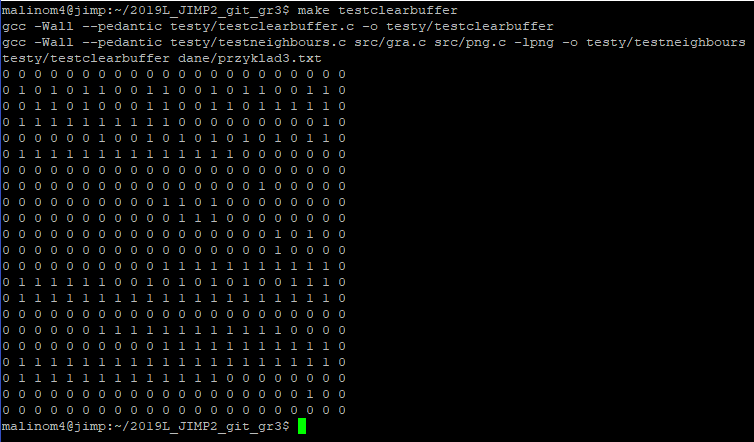
\includegraphics[width=14cm]{obrazy/testbuffer.png}
\caption{Test clear\_buffer()}
\label{test clear_buffer}
\end{figure}
\item Drugi miniprogram, \code{testneighbours} służy do przetestowania działania funkcji \code{neighbours()}  i po uruchomieniu wyświetla liczbę żywych sąsiadów każdej komórki w podanym pliku.\par
Przykład:
\begin{figure}[H]
\centering
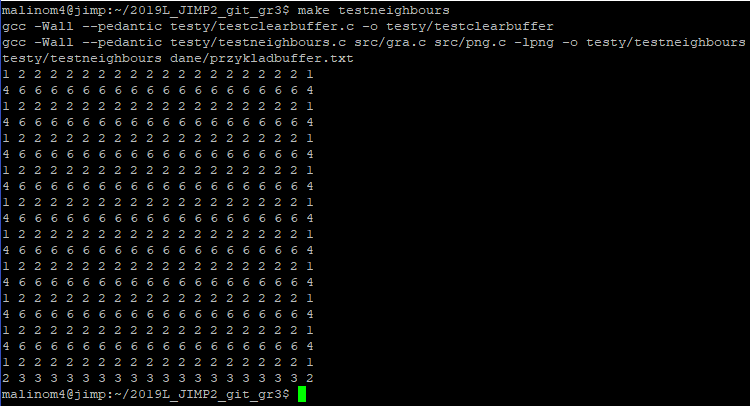
\includegraphics[width=14cm]{obrazy/testneighbours.png}
\caption{Test neighbours()}
\label{test neighbours}
\end{figure}
\item Moduł \code{png.c} przetestowano generując obrazy z generacji i porównując je ręcznie.\par
Przykład:
\begin{figure}[H]
\centering
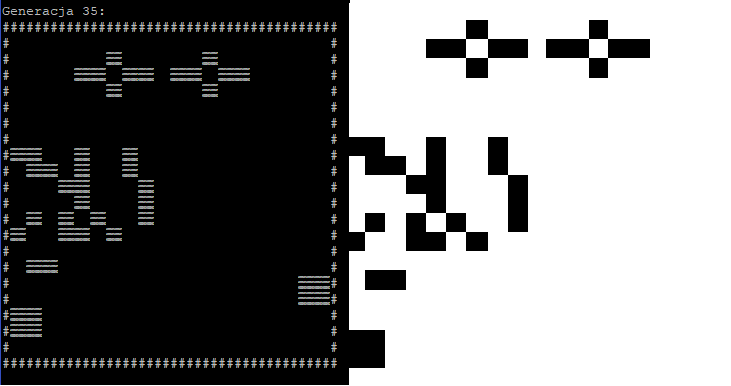
\includegraphics[width=14cm]{obrazy/testpng.png}
\caption{Test PNG}
\label{test png}
\end{figure}
\item Funkcję \code{make\_generation()} przetestowano uruchomiając program dla specjalnie przygotowanych danych zawierających wzory o znanych ruchach takich jak kwadrat, ul oraz sygnalizator.\par
Przykład:
\begin{figure}[H]
\centering
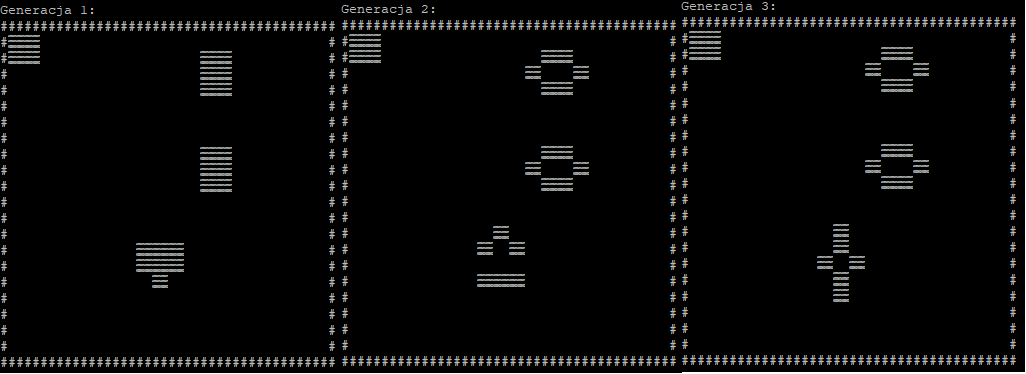
\includegraphics[width=14cm]{obrazy/testmakegen.png}
\caption{Test make\_generation()}
\label{test make_generation}
\end{figure}
\item Funkcję \code{check\_filename()} przetestowano podając jej błędne nazwy pliku i~potwierdzając że je odrzuciła.\par
Przykład:
\begin{figure}[H]
\centering
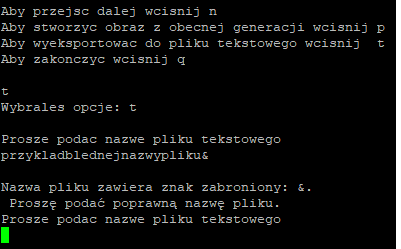
\includegraphics[width=14cm]{obrazy/testcheckname.png}
\caption{Test check\_filename()}
\label{test check_filename}
\end{figure}
\item Moduł \code{sterowanie.c} przetestowano podając mu argumenty i potwierdzając, że odrzuca błędne a przyjmuje poprawne.\par
Przykład:\par
\begin{figure}[H]
\centering
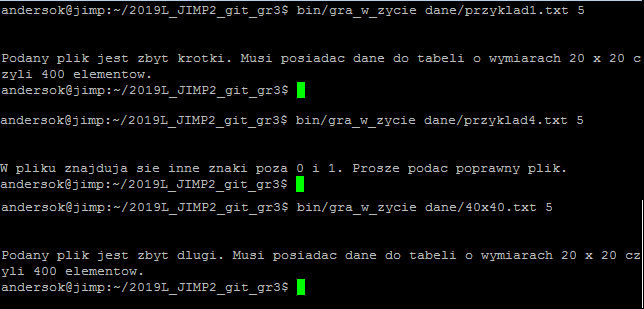
\includegraphics[width=14cm]{obrazy/teststerowanie.png}
\caption{Test sterowania}
\label{test sterowanie}
\end{figure}
\end{enumerate}
\end{document}





